\section{Northern Hemisphere Data Pipeline}

\subsection{Data Format}

The final data output will be a full sky map presented in Healpix format as described by \citeasnoun{Calabretta2007}. This is a method of pixellating the sky into equal area pixels, and is commonly used in sky maps (for example WMAP).



\subsection{Data Pipeline}

% The switched signal (illustrated in \fign{fig:pseudo_correlation}) is sampled by an Analog-to-digital convertor (ADC) and 10~ms integrations performed by a field programmable gate array (FPGA). From the switched data it is possible to determine the the $T_{sky}$ - $T_{load}$ signal from the total intensity channels. The polarisation channels provide measurements of Stokes Q and U.

The data pipeline is currently being developed with the the processes (in rough sequence) including:

\begin{enumerate}
 \item Deglitching
 \item RFI excision
 \item 60Hz Mains Removal
  \item $\alpha$ correction for polarisation channel leakage 
 \item r factor correction to account for imbalance in temperature between cold load and sky (see \cite{Mennella:2003ii}
 \item Cold load corection fits for a sinusoidal (amplitude 1.9mK, frequency 1.2Hz) variation in the cold load temperature 
 \item Atmospheric Opacity Corrections
\end{enumerate}


An in depth discussion of these corrections is beyond the scope of this report. It is important to note that many of the steps listed, can be applied using different methods, with the optimal strategy is currently being decided upon. 

The data pipeline outlined above is implemented in MATLAB. Suitably calibrated and cleaned data is then written to FITS files, and passed on to the \textit{Descart} mapping suite (reference?). This suite of software is capable of destriping (extracting a 'true' signal for each pixel using multiple observations with different telescope parameters), however we are currently not utilising the functionality and are rather operating in the \textit{naive} software mode. This simply subtracts a mean bias offset, and averages the signal per Healpix pixel.

A current skymap of the data taken from OVRO is included in \fign{fig:northSkySurvey}. The map (in galactic coordinates) shows evidence of non-uniform scanning (around the North Celestial Pole) and also clearly shows the work that is still required in calibrating the data. However, the map does show the galactic plane as well as more detailed structure. This is a positive early stage C-BASS result, although there remains considerable work to be done.



\begin{figure}
 \centering
 %\subfloat[Northern sky as measured by the OVRO antenna-low contrast]{\includegraphics[width=0.4\textwidth,height=0.25\textheight]{images/maps/5GHz_2.jpg}}
%\hspace{0.1cm}
 %\subfloat[Northern sky simulated by Clive Dickinson- approximately same colour scale as in (a) ]{\includegraphics[width=0.4\textwidth,height=0.25\textheight]{images/maps/5GHz_coadded_500.jpg}}\\
 \subfloat[Increasing the contrast of the OVRO data shows significant calibration issues]{\includegraphics[width=0.4\textwidth,height=0.25\textheight]{images/maps/5GHz_02.jpg}}
\hspace{0.1cm}
 \subfloat[The simulated map on a similar intensity scale as in (c) shows the structure that we expect]{\includegraphics[width=0.4\textwidth,height=0.25\textheight]{images/maps/5GHz_coadded_80}}

 % newdish_upgrade.jpg: 1280x728 pixel, 72dpi, 45.16x25.68 cm, bb=
 \caption{Current state of Northern Sky maps (in Galactic Coordinates). Note that since we haven't yet introduced an absolute calibration scale, the comparisons between our data and simulated data are approximate.}
 \label{fig:northSkySurvey}
\end{figure}

% \begin{figure}
%  \centering
%  \includegraphics[width=\textwidth]{./images/descart/destriping.png}
%  % destriping.png: 1920x1200 pixel, 72dpi, 67.73x42.33 cm, bb=0 0 1920 1200
%  \caption{Illustration of destriping data (Joe Zuntz private communication)}
%  \label{fig:destriping}
% \end{figure}


 

\subsection{Noise Diode Stability and Linearity}

\fign{fig:northSkySurvey} shows the importance of proper calibration. Many of the choices available to us in calibrating the data rely on injecting a well understood noise diode signal. The long term stability of the noise diode is particularly important in this.

To this end we have begun a process of monitoring the noise diode against bright calibration sources. The resulting data from scans against CasA and TauA are shown in \fign{fig:calCheck}. These scans have been optimised to allow the following checks:

\begin{enumerate}
 \item Noise Diode linearity
 \item Pointing
 \item Noise diode stability
 \end{enumerate}

The noise diode linearity is easily check by comparing the noise diode contribution to the signal while off source, against the contribution while on source. If the noise diode is in a linear region, the relative contributions should be the same. Pointing is checked by fitting a gaussian to the azimuth and elevation cross scans. This pointing 'sanity' check is critical, as even small pointing errors will effect the measured flux, and hence our ability to check the noise diode stability. For the stability we can simply compare the noise diode signal to source signal over a period of time. Since the time between the noise diode event and calibration scan is short, any variations in receiver gain or atmospheric contributions are  common to both. 


\begin{figure}
 \centering
\subfloat[CasA used to check detector diode linearity and long term stability of the noise diode]{\includegraphics[width=\textwidth,height=0.7\textheight]{./images/calibration/casALabelled.pdf} \label{fig:casACal}}
\hspace{0.2cm}
%\subfloat[TauA used to check detector diode linearity and long term stability of the noise diode]{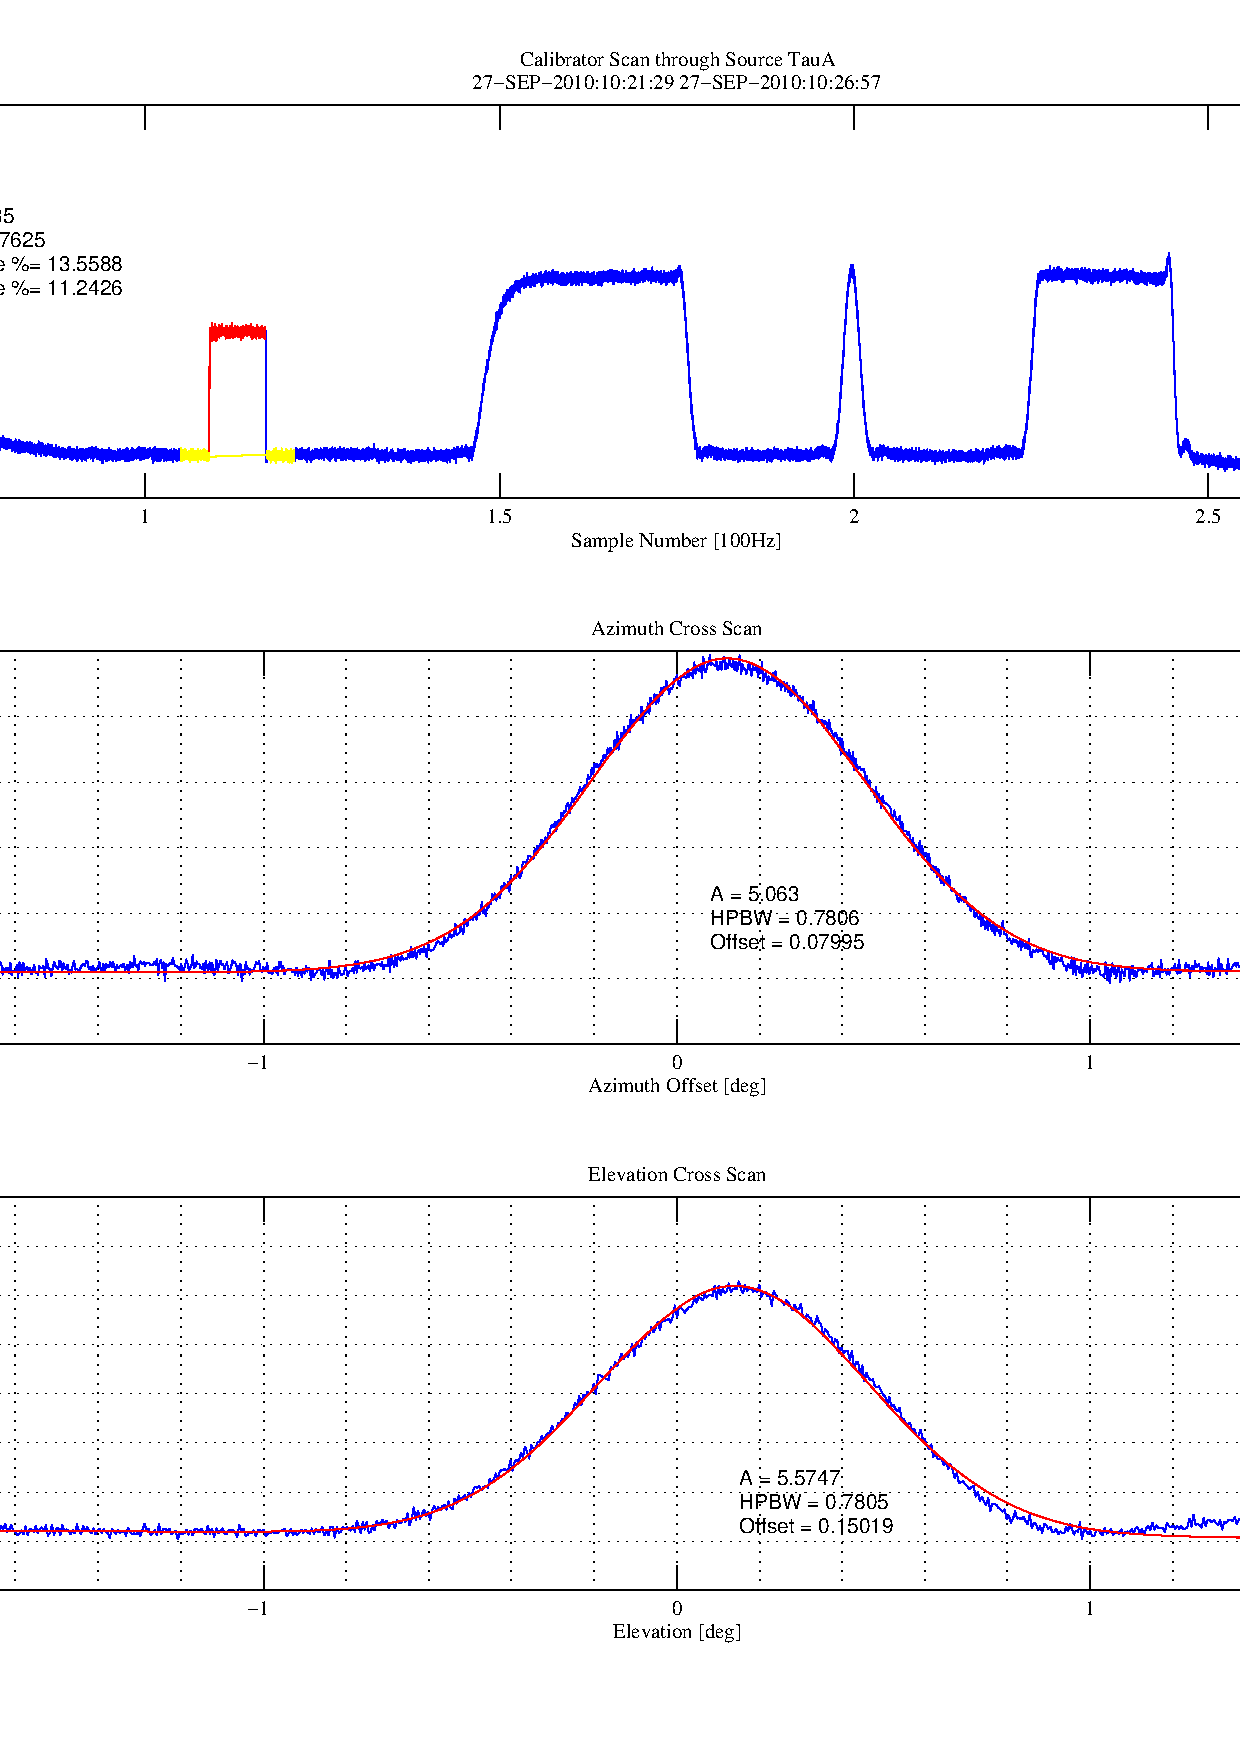
\includegraphics[width=\textwidth,height=0.35\textheight]{./images/calibration/tauA.pdf} \label{fig:tauACal}}
\caption{Long term noise diode stability observations. These show the check for the linearity of the detector diode (\textit{Diode Slope}) by comparison between the two noise diode events and the antenna pointing check performed on  the CasA. This is a bright, point sources in the 0.8$^{\circ}$ C-BASS beam. This shows evidence for detector diode non-linearity, with the slope of the diode output decreasing by $\approx$ 2.7\%. The first noise diode event is triggered with the telescope at the same elevation as the source but with an offset of 5$^{\circ}$ in azimuth. If the time between Noise Diode Event \#1 and the azimuth cross scan is short and at the same elevation as the source (i.e receiver gain fluctuations and atmospheric effects are negligible), and the pointing is accurate, it is possible to calibrate the noise diode signal against the source, and check the long term stability of the noise diode.  }
\label{fig:calCheck}

\end{figure}




